Image Diffusion Models were first introduced by SohlDickstein et al. 
\cite*{Sohl-Dickstein2015,kingma2021variational} and have been recently applied to
image generation \cite*{dhariwal2021diffusion,}. The Latent Diffusion Models
(LDM) \cite*{LDM} performs the diffusion steps in the latent image
space [19], which reduces the computation cost. Text-toimage diffusion models achieve state-of-the-art image generation results by encoding text inputs into latent vectors
via pretrained language models like CLIP \cite*{CLIP}. Glide \cite*{glide}
is a text-guided diffusion model supporting image generation and editing. Disco Diffusion [5] processes text prompts
with clip guidance. Stable Diffusion \cite*{stablediffusionv15} is a large-scale
implementation of latent diffusion \cite*{LDM}. Imagen \cite*{saharia2022photorealistic} directly
diffuses pixels using a pyramid structure without using latent
images. Commercial products include DALL-E2 \cite*{openai2023dalle2} and
Midjourney \cite*{midjourney2023}.




\subsection{Exploration of Denoising Diffusion Probabilistic Models}

Denoising Diffusion Probabilistic Models (DDPMs) \cite*{DDPM} introduce an innovative framework for generative models that emphasize the reverse engineering of diffusion processes. These models utilize parameterized Markov chains to methodically transform noise into organized patterns over multiple iterations.

The diffusion phase commences with an initial distribution \(x_0 \sim q(x_0)\), methodically incorporating Gaussian noise over \(T\) timesteps. At each step \(t\), the noising process is characterized by:
\begin{equation}
q(x_{1:T}|x_0) = \prod_{t=1}^{T} q(x_t|x_{t-1}),
\end{equation}

\begin{equation}
q(x_t|x_{t-1}) = \mathcal{N}(x_t; \sqrt{1-\beta_t}x_{t-1}, \beta_t\mathbf{I}),
\end{equation}
where \( \beta_t \) represents the stepwise noise variance parameters.

In the denoising phase, DDPMs aim to incrementally cleanse the data, effectively reversing the diffusion sequence. This begins from a noisy state \(x_T\) and progressively works towards the initial data distribution \(q(x_0)\). The model specifies the reverse transition \(p_{\theta}(x_{t-1}|x_t)\) with:
\begin{equation}
p_{\theta}(x_{t-1}|x_t) = \mathcal{N}(x_{t-1}; \mu_{\theta}(x_t, t), \Sigma_{\theta}(x_t, t))
\end{equation}
Deep learning models, notably those based on UNet architectures, parameterize \( \mu_{\theta}(x_t, t) \) and \( \Sigma_{\theta}(x_t, t) \). These models input the noised data \(x_t\) and timestep \(t\), predicting the normal distribution's parameters to identify the noise \( \epsilon_{\theta} \) needed for reversing the diffusion. Generating new data instances \(x_0\) involves starting with a noise vector \(x_T \sim p(x_T)\) and sequentially sampling from \(p_{\theta}(x_{t-1}|x_t)\) until \(t=1\), completing the reverse diffusion pathway.

The methodologies underlying the training and sampling of DDPMs are elucidated through pseudocode in the referenced Algorithm \ref{alg:ddpm_training} and Algorithm \ref{alg:ddpm_sampling}. These algorithms detail the procedural steps for both learning the model parameters and generating new samples, providing a comprehensive understanding of the operational framework of DDPMs.


\begin{algorithm}
    \caption{DDPM Training}\label{alg:ddpm_training}
    \begin{algorithmic}[1]
    \Repeat
        \State $x_0 \sim q(x_0)$
        \State $t \sim \text{Uniform}\{1, \ldots, T\}$
        \State $\varepsilon \sim \mathcal{N}(0, I)$
        \State Take gradient descent step on
        \State $\nabla_\theta \left\| \varepsilon - \varepsilon_\theta(\sqrt{\alpha_t}x_0 + \sqrt{1 - \alpha_t} \varepsilon, t) \right\|^2$
    \Until{converged}
    \end{algorithmic}
    \end{algorithm}
    
\begin{algorithm}
    \caption{DDPM Sampling}\label{alg:ddpm_sampling}
    \begin{algorithmic}[1]
    \State $x_T \sim \mathcal{N}(0, I)$
    \For{$t = T, \ldots, 1$}
        \State $z \sim \begin{cases} 
        \mathcal{N}(0, I) & \text{if } t > 1 \\
        0 & \text{else}
        \end{cases}$
        \State $x_{t-1} = \frac{1}{\sqrt{\alpha_t}} \left(x_t - \frac{1-\alpha_t}{\sqrt{1 - \alpha_t}} \varepsilon_\theta(x_t, t)\right) + \sigma_t z$
    \EndFor
    \State \Return $x_0$
    \end{algorithmic}
    \end{algorithm}

\begin{figure}[h!]
    \centering
    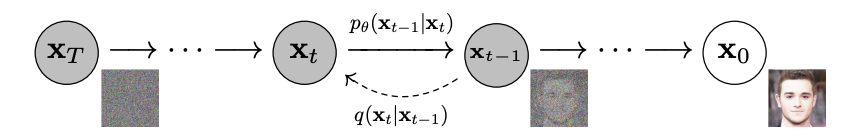
\includegraphics[width=\textwidth]{images/DDPM.png}
    \caption{Mind Map of diffusion models \cite*{DDPM}}
\end{figure}